\section{Detalles de Implementación y Pruebas}

En este punto la teoría y la implementación de los diferentes algoritmos se
pasan por diversas pruebas, que medirán su fidelidad, consistencia y
efectividad, para
que así astrónomos o investigadores, con toda confianza puedan explotar la
información
que tienen, automatizando las acciones y optimizando el tiempo dedicado al
análisis.
Las pruebas son llevadas a cabo en una computadora portátil marca Apple,
modelo Macbook Air, la cual cuenta con un procesador de 1.6 Ghz Intel Core i5,
Memoria DDR3 de 2 GB y 1333 MHz, Gráficos Intel HD Gráficos 3000 288 MB y
sistema operativo Maverick versión 10.9.3.
En primera instancia se prueban uno a uno los módulos testeando si realizan
correctamente lo esperado y a su vez los tiempos de respuesta. En cada etapa del
registro
se ingresan diferentes parámetros de entrada y su consistencia en ellos. Los
módulos
están separados en dos tipos: Módulos superiores, que corresponden a todos
aquellos
que son protagonistas en las etapas del registro y módulos inferiores que
realizan tareas
de cálculo que colaboran con los módulos superiores.

\subsection{Módulos Superiores}

En esta etapa se probarán los módulos por separado, midiendo su
efectividad, consistencia de la información y el tiempo de procesamiento para
diferentes
cantidades de imágenes. Se irán mostrando tablas comparativas en cada tipo de
algoritmo y los resultados visuales obtenidos. Para poder visualizar los
resultados de
cada imagen, se ha utilizado DS9, software que permite entre muchas cosas ver
una
imagen. La imagen de a continuación corresponde a la Galaxia Lenticular NGC
5128, la
cual fue capturada por el Telescopio Schmidt del Reino Unido, tiene dos
dimensiones
las cuales son de 1095 x 1095, esta será utilizada para las diferentes pruebas
llevadas a
cabo.

\subsubsection{Recortar}
Módulo que tiene como entrada un vector de coordenadas (x,y), las cuales
representan el borde del objeto elíptico y la matriz de información de la imagen
que contiene el objeto. El sistema recorre punto a punto determinando el mayor y
menor valor en ‘x’ y en ‘y’, los cuales definen el límite de la zona en donde se
encuentra el objeto. Las imágenes de a continuación, figura 4-2, 4-3 y 4-4,
representan una imagen de forma matricial la cual posee un objeto elíptico.


La tabla de a continuación detalla la salida obtenida al ingresar las matrices
anteriormente mas el vector de coordenadas.

El tiempo de procesamiento es bastante rápido en general, si en una matriz de
10x10
tarda en promedio 0.00014456 segundos, comportamiento casi constante, en una
matriz
de 2000 x 2000, siguiendo el mismo comportamiento lineal se puede estimar que no
tardaría mas de 1 segundo en hacer una extracción.
Las imágenes de a continuación, figura 4-4, 4-5 y 4-6 representan la matriz de
entrada
ingresada al sistema y su respectiva salida.

\subsubsection{Rotación}

Modulo que tiene como entrada la matriz que se desea rotar, su dimensión, y el
ángulo en el cual será rotada. El módulo retorna la matriz rotada en el ángulo
respectivo en sentido antihorario.

Mirando la table se puede apreciar, que el tiempo de computo en procesar una
rotación de 90o es mas rápido que los otros ángulo, un 12 segundos contra 15 que
tarda una rotación en 5o, esto se puede entender dado que cuando la matriz es
rotada en 90o*n, con n pertenecientes a los cardinales, las coordenadas rotadas
siempre caerán en valores enteros, por lo que no será necesario interpolar la
información. Independiente de eso, en interpolar solo se invierte 3 segundos. No
siempre será necesario rotar la imagen, por lo que se puede decir, que rotando
una muestra de 100, el astrónomo invertirá aproximadamente 1225 segundos si
el programa no necesita interpolar.
A continuación se muestran los resultados visuales para una rotación de 5, 45,
73
y 128 grados. Ver figura 4-8, 4-9, 4-10 y 4-11.

\subsubsection{Escalar}
Modulo que tiene como entrada la matriz que se desea rotar, su dimensión, y la
razón en que será escalada. Para notar la diferencia se mostrará la imagen
escalada con y sin interpolación. Cuando termina la ejecución, el módulo retorna
la matriz escalada.

Observando la tabla se puede apreciar la diferencia tajante de cuando una imagen
es ampliada o no, por ejemplo, cuando se amplía en una razón de dos se
requieren casi 25 segundo para que se lleve a cabo, en cambio cuando la imagen
se achica en una razón de 1\/4, tan solo se necesitan 12.75 segundos, esta
diferencia surge dado que no es necesario crear información intermedia entre
puntos. A medida que crece la taza de ampliación, es mas costoso el tiempo de
procesamiento. La imagen de a continuación representa una ampliación para una
razón de 2 sin interpolar, en ella se puede apreciar como los puntos al
distribuirlos quedan sin información entre ellos.

Si viéramos esta misma imagen mas de cerca, apreciaríamos que los puntos están
uniformemente distribuidos, y a dos puntos de distancia, figura 4-13, hay un
nuevo punto con información. Si la razón fuera 5, figura 4-14, los puntos
estarían
aún mas disperso.

Cuando la imagen se agranda el algoritmo entra en una segunda fase, que
consiste en completar la información vacía, la cual es la parte más costosa del
algoritmo,
ya que se invierte mínimo el 92\% del tiempo, con una tendencia creciente muy
marcada.

La tabla 4.3 muestra como influye en el tiempo de respuesta la interpolación. El
tiempo
sin interpolar es insignificante y casi invariante el tiempo de escalar.

Acontinuación, figura 4-15, se puede apreciar el resultado de la imagen escalada
e
interpolada.

\subsubsection{Alinear}
El módulo alinear tiene como entrada la coordenada del punto central del objeto
en la imagen de referencia, del objeto de la imagen actual, la dimensión de la
imagen de de referencia y de la imagen actual, y la matriz de información de la
imagen actual. Este módulo retorna una matriz de tamaño igual a la de
referencia, con el objeto de la imagen actual centrado en el mismo punto que el
objeto de referencia. Este proceso no requiere de mucho tiempo de ejecución ya
que básicamente es trasladar puntos.

\subsubsection{Deproyectar}
El siguiente módulo tiene como entrada el punto (x,y) donde se llevará el centro
del objeto actual, la dimensión de la imagen de referencia, las coordenadas del
borde del objeto que se esta analizando, su matriz de información y el radio.

El efecto logrado en la imagen no ha sido muy notorio, dado que el objeto ya
poseía una forma circular. El tiempo de ejecución no es muy alto a pesar de la
cantidad de puntos que se deben interpolar. La figura 4-10 muestra como una
serie de puntos fueron trasladados una distancia igual al radio del objeto, en
sentido parametrico de la circunferencia.

\subsection{Módulos Inferiores}
Esta etapa de pruebas consiste en validar el sistema de cómputo oculto dentro
del
sistema, que colabora colabora con los módulos superiores entregando información
vital
de los objetos en las variadas imágenes antes de realizar cualquier
transformación
geométrica en el plano.

\subsubsection{Distancia entre puntos}

Función que tiene como entrada dos coordenadas (X 1 ,Y 1 ) y (X 2 ,Y 2 ), de las
cuales
calcula su distancia lineal. Se prueban diferentes valores para ‘X’ e ‘Y’. Por
cada
resultado se tomará el tiempo de cálculo.
La tabla 4.7, para las diferentes entradas de (X,Y) se muestra su distancia, y
el
tiempo en segundo que tarda en calcularla.

\subsubsection{Medida del eje mayor}
Algoritmo que a partir de un vector que se compone de todas las coordenadas
que son parte del borde del objeto elíptico, determina cual es la mayor
distancia
entre ellas. El vector se recibe de la siguiente manera, tabla 4.8:

A continuación probaremos tres objetos elípticos, figura 4-18, figura 4-19 y
figura 4-20. La tabla

\subsubsection{Ángulo a rotar}
Función que recibe como parámetros de entrada las coordenadas del borde de la
elipse, retornando el complemento del ángulo de la pendiente.

\subsubsection{Centro geométrico}
Función que recibe como parámetros de entrada el tamaño del eje mayor del
objeto, sus coordenadas y la pendiente de la recta, entregando como salida, las
coordenadas del centro del objeto.


%\subsection{Definiciones básicas}
%
%Para llevar a cabo la normalización se han definido cuatro etapas
%(Fig.~\ref{img:represent}) en las que son ajustadas un conjunto de
%imágenes a un formato general antes de ser analizadas. Se entiende que
%en cada imagen existe el mismo objeto de estudio, pero puede variar su
%posición, tamaño y forma. Al ir procesando cada imagen, se van
%aplicando los filtros respectivos, los cuales permiten que las
%imágenes queden con un patrón común que facilite su estudio. El
%siguiente esquema visualiza cómo se desarrolla el proceso de
%normalización en un conjunto de imágenes:
%
%\begin{figure}[hb!]
%  \begin{center}
%    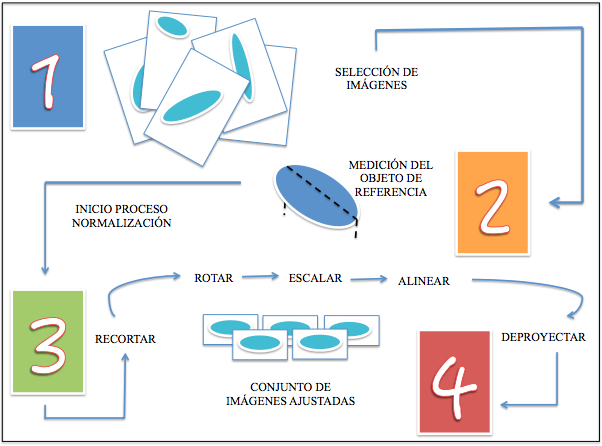
\includegraphics[scale=.5]{image/representacion}
%  \end{center}
%  \caption{Representación del proceso para registrar una
%  imagen.}\label{img:represent}
%\end{figure}
%
%\begin{enumerate}[I]
%  \item El diagrama parte con la selección de imágenes que poseen objetos
%    que al usuario le interesa estudiar. Una de estas imágenes será tomada
%    como referencia para realizar el ajuste de las restantes. 
%  \item Cada vez que una imagen es leída por el programa, éste realiza la
%    toma de medidas, es decir, la longitud del eje mayor del objeto y su
%    ángulo de proyección respecto a un eje horizontal. 
%  \item Luego, pasa por cinco etapas de ajuste,  extracción del objeto de
%    interés, rotación del objeto con respecto al eje mayor, el cual se
%    deja sin pendiente, luego se escala y se alinea en relación a la
%    imagen de referencia, 
%  \item para que finalmente, se pueda deproyectar, transformando la elipse
%    en un círculo.
%\end{enumerate}
%
%Cada nivel de ajuste contempla el ingreso de información externa
%respecto a la posición actualizada del objeto, es decir, se necesita
%saber antes y después de realizar el ajuste en qué coordenadas va
%quedando el objeto. Cabe destacar que todos los algoritmos realizados
%para cada etapa de ajuste, exceptuando la deproyección, pueden ser
%empleados en cualquier tipo de objeto astronómico, ya sean galaxias,
%cúmulos globulares, nebulosas, etcétera, y para fines de esta memoria
%se trabajó puntualmente en la deproyección de objetos elípticos.
%
%
%
%\subsection{Preparación de la información}
%
%Corresponde en esta instancia seleccionar diversos objetos con forma
%similar a una elipse, a los cuales se les realizan transformaciones
%geométricas en el plano (Fundación Polar). En este proceso, se
%selecciona una imagen de referencia con la cual se trabaja para llevar
%a cabo la normalización. Los objetos elípticos a manipular
%corresponden a galaxias que presentan una forma elíptica.
%
%Es esencial conocer en cada etapa las coordenadas que componen el
%borde de la elipse, lo que ayuda a procesar la información útil dentro
%de la imagen, determinar la medida del eje mayor e inclinación de esta
%pseudo elipse. Es aquí donde se puede  determinar que tan grande o
%tanto más pequeña es del resto, como también saber su ángulo de
%rotación respecto al eje horizontal y su medida de deproyección, es
%decir, lo que le falta a la elipse para transformarla en círculo.
%
%Entiéndase que una elipse es una curva simétrica cerrada, que se
%obtiene al cortar la superficie de un cono con un plano oblicuo al eje
%de simetría, en palabras mas sencillas, es como un circunferencia
%estirada simétricamente. En una elipse, se puede identificar el eje
%mayor, como los puntos que están más distantes entre sí, los cuales se
%determinan calculando las diferencias que existen entre los puntos
%correspondientes al borde de la elipse.  Para saber la distancia entre
%dos puntos en un plano, es utilizado el ``Teorema de Pitágoras''
%(\ref{eq:tp}), el cual dice, que la suma de los catetos al cuadrado es
%igual a la hipotenusa al cuadrado, que en este caso es la distancia
%entre dos puntos de la elipse, como lo muestra la Fig.~\ref{img:tp}.
%
%\begin{align}
%  a^2 & = b^2 + c^2 \label{eq:tp}
%\end{align}
%
%\begin{figure}[hb!]
%  \begin{center}
%    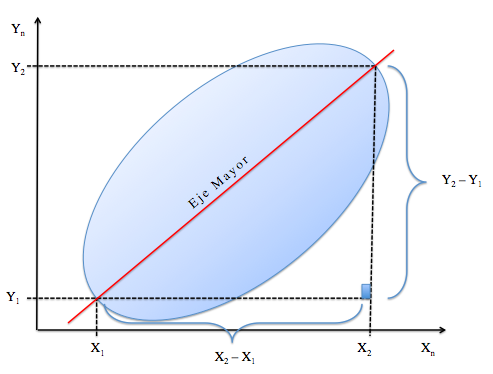
\includegraphics[scale=.5]{image/calculoEje}
%  \end{center}
%  \caption{Cálculo del eje mayor de la elipse.}\label{img:tp}
%\end{figure}
%
%Matemáticamente, la expresión que calcula la distancia entre dos
%puntos se escribe (\ref{eq:distancia}):
%
%\begin{align}
%  \text{eje mayor} & = \sqrt{\left(x_2 - x_1\right)^2 + \left(y_2 -
%  y_1\right)^2} \label{eq:distancia}
%\end{align}
%
%Conociendo la distancia del eje mayor, se procede a determinar su
%ángulo en relación al eje horizontal del plano. Esto, permite
%reconocer en que medida rotar el objeto antes de ser comparado. Para
%encontrar el ángulo de rotación, basta calcular la inversa de la
%función tangente (\ref{eq:tangente}), en la que, aplicando el arco
%tangente a la razón existente entre la diferencia de los puntos en el
%plano vertical, dividida por la diferencia de los puntos en el plano
%horizontal, da como resultado, el ángulo de la recta. Gráficamente se
%puede apreciar en la Fig.~\ref{img:tangente}.
%
%\begin{align}
%  \partial & = \tan^{-1}\left(\frac{Y_{2-Y_1}}{X_{2-X_1}}\right)
%  \label{eq:tangente}
%\end{align}
%
%\begin{figure}[hb!]
%  \begin{center}
%    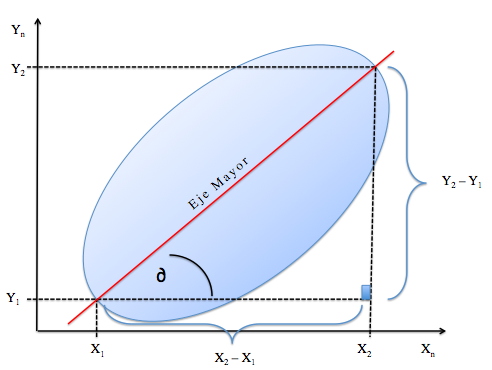
\includegraphics[scale=.5]{image/detAngulo}
%  \end{center}
%  \caption{Determinación del ángulo de proyección del eje mayor de la
%  elipse con respecto al eje horizontal del plano.}\label{img:tangente}
%\end{figure}
%
%El punto centro de la elipse, permite ajustar el resto de los objetos
%a ese punto de referencia. Para definir el punto, basta con dividir el
%eje mayor en dos y estimar a que coordenada corresponde. Para
%identificar la posición que ocupa en el plano el centro del objeto, se
%le suma a una de las coordenadas, que pertenece a la esquina del eje
%mayor, la proyección de la mitad de este eje.
%
%Para saber la posición en el plano del centro del objeto se toma una
%esquina del eje mayor como referencia y se le suma tanto en el eje $x$
%(eje horizontal) como en el eje $y$ (eje vertical) la proyección de la
%mitad del eje mayor. La expresión matemática (\ref{eq:distX}) y
%(\ref{eq:distY}) corresponden al cálculo de la distancia en los dos
%ejes del plano.
%
%\begin{align}
%  \text{distancia en eje } x & = \cos{\left(\partial\right)} * \text{
%  distancia eje mayor } * 0.5 \label{eq:distX}\\
%  \text{distancia en eje } y & = \sin{\left(\partial\right)} * \text{
%  distancia eje mayor } * 0.5 \label{eq:distY}
%\end{align}
%
%Una vez reconocida la distancia del eje respecto al punto menor ya es
%posible determinar la coordenada del punto central. La expresión
%(\ref{eq:sumaDist}), suma estas distancias a la coordenada menor del
%eje obteniendo así el punto central del objeto.
%
%\begin{align}
%  \text{punto central eje} & = \left(X_1 + \text{ distancia en eje }
%  x, Y_1 + \text{ distancia en eje } y\right) \label{eq:sumaDist}
%\end{align}
%
%Gráficamente, lo podemos apreciar en la Fig.~\ref{img:puntoCentral}.
%
%\begin{figure}[hb!]
%  \begin{center}
%    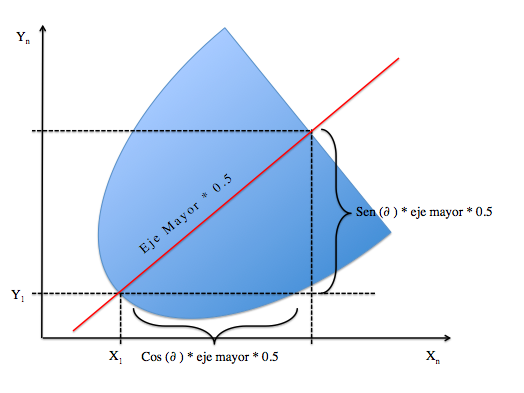
\includegraphics[scale=.5]{image/puntoCentral}
%  \end{center}
%  \caption{Cálculo del punto central de la
%  elipse.}\label{img:puntoCentral}
%\end{figure}
%
%Los mecanismos antes expuestos desde el punto de vista algorítmico se
%detallan en la siguiente sección.
%
%
%
%\subsection{Prototipado para proceso de normalización}
%
%La normalización define cinco etapas:
%
%\begin{itemize}
%  \item Extraer de la imagen el objeto de interés.
%  \item Rotar el objeto dejándolo paralelo al eje horizontal.
%  \item Escalar el objeto dejándolo del mismo tamaño que el objeto de
%    referencia.
%  \item Alinear el objeto a un punto de referencia común.
%  \item Deproyectar el objeto hasta que quede como un círculo.
%\end{itemize}
%
%\paragraph{Algoritmo recorte}
%
%Para extraer de la imagen el objeto de interés, descartando todo el
%resto de la información que no es necesaria, se debe recortar la
%imagen y así trabajar solo con la información útil, lo que permite
%realizar sólo los cálculos necesarios, entregando la información más
%precisa. Al realizar la observación de una determinada ubicación en el
%espacio, puede ocurrir que la imagen posea más de un objeto, pero el
%foco de interés radica en uno solo de ellos, en este caso, es
%sumamente útil individualizar y concentrar el estudio en la
%información que se necesita descartando el resto. Para recortar la
%imagen se debe determinar los puntos extremos del cuerpo elíptico, es
%decir, mirándolo desde el punto matricial, encontrar el mayor y el
%menor valor de la fila y columna. Para esto, se recorre el borde del
%objeto hasta encontrar los cuatro puntos. El algoritmo
%(\ref{alg:extraccion}) que se presenta a continuación realiza la
%extracción.
%
%\begin{algorithm}
%\caption{Algoritmo recorte.}
%\label{alg:extraccion}
%\begin{algorithmic}[1]
%\STATE Función recortar$($matriz, borde$)$:
%\STATE fila\_mayor = 0
%\STATE file\_menor = borde[0]
%\STATE columna\_mayor = 0
%\STATE columna\_menor = borde[1]
%\STATE $i = 0$
%\WHILE{$i != $ largo(borde) - 1}
%\IF{$i$ es impar}
%\STATE continúe
%\ENDIF
%\IF{fila\_mayor $<$ borde[$i$]}
%\STATE fila\_mayor = borde[$i$]
%\ENDIF
%\IF{fila\_menor $>$ borde[$i$]}
%\STATE fila\_menor = borde[$i$]
%\ENDIF
%\IF{columna\_mayor $<$ borde[$i + 1$]}
%\STATE columna\_mayor = borde[$i + 1$]
%\ENDIF
%\IF{columna\_menor $>$ borde[$i + 1$]}
%\STATE columna\_menor = borde[$i +  1$]
%\ENDIF
%\ENDWHILE
%\STATE $i = 0$
%\WHILE{$i != $ largo(borde) - 1}
%\IF{$i$ es impar}
%\STATE continúe
%\ENDIF
%\STATE borde[$i$] = borde[$i$] - fila\_menor
%\STATE borde[$i + 1$] = borde[$i + 1$] - columna\_menor
%\STATE $i$ = fila\_menor
%\ENDWHILE
%\WHILE{$i != $ fila\_mayor + 1}
%\STATE $j = $ columna\_menor
%\WHILE{$j != $ columna\_mayor + 1}
%\STATE matriz\_final[$i$ - fila\_menor][columna\_menor] = matriz[$i$][$j$]
%\ENDWHILE
%\ENDWHILE
%\STATE retorno matriz\_final
%\end{algorithmic}
%\end{algorithm}
%
%En las líneas 2, 3, 4 y 5, se declaran las variables que guardarán el
%menor y mayor valor entre las filas y columnas que pertenecen al borde
%del objeto de estudio, nótese que no es identificar el valor existente
%en la posición, sino la posición en si. De la línea 11 a la 21, se
%encuentra el valor para fila\_mayor, fila\_menor, columna\_mayor y
%columna\_menor. Finalmente de la línea 24 a la 36, se traslada el
%objeto de manera tal, que los valores encontrados para fila y columna,
%sean el borde la imagen.
%
%\paragraph{Algoritmo de rotación \ref{alg:rotacion}}
%
%La rotación consiste en girar un objeto en torno a punto. Por cada
%imagen que ingresa se calcula su ángulo de proyección respecto al eje
%horizontal para que posteriormente se rote en esta medida hasta que el
%ángulo sea cero, dado que es más sencillo dejar bajo la misma
%pendiente que tratar de hacer coincidir a una de referencia.
%
%Como en la toma de medidas, el ángulo está determinado, en esta etapa
%se da la orden de rotar en sentido antihorario el complemento del
%ángulo. 
%
%Una imagen es básicamente una matriz de $n$ filas y $m$ columnas, con
%posiciones del $(0,0)$ al $(n-1, m-1)$. Para poder rotarla se
%multiplica una matriz de rotación definida con seno y coseno por cada
%coordenada. Antes de rotar la imagen, existen algunos ángulos (90, 180
%y $270^\circ$), en donde no es necesario multiplicar las coordenadas de la
%matriz imagen por la matriz de rotación, tan solo es necesario hacer
%una traslación de puntos.  
%
%Cuando el ángulo a rotar es diferentes a los antes expuestos, recién
%se utiliza la matriz de rotación. Cabe destacar, que la rotación se
%realiza en torno al origen, es decir, el punto $(0,0)$, entonces antes
%de girar la imagen, se debe trasladar el centro del objeto a ese
%punto. Esto ocurre básicamente por la forma en que está definida la
%matriz de rotación (Ec.~\ref{eq:matrixRot}).
%
%\begin{align}
%\begin{pmatrix}
%  \cos{\partial} & -\sin{\partial} \\
%  \sin{\partial} & \cos{\partial}
%\end{pmatrix}\label{eq:matrixRot}
%\end{align}
%
%Para evitar que alguna posición de la matriz quede negativa, se
%traslada el centro del objeto al origen, se rota y se vuelve a dejar
%en un cuadrante positivo. Para esto se debe saber cual es el centro
%del objeto, de modo de desplazar todos los puntos en esa medida, luego
%se rota identificando el punto más negativo. Esta medida sirve para
%desplazar en esa cantidad todas las coordenadas a un eje positivo.
%
%\begin{algorithm}
%\caption{Algoritmo de rotación.}
%\label{alg:rotacion}
%\begin{algorithmic}[1]
%\STATE Funcion rotar (matriz, NAXIS1, NAXIS2, ángulo):
%\IF{ángulo $>$ 360 OR ángulo $<$ 1}
%\STATE imprimir ''$<$Error: Imagen no rotada, ángulo no permitido$>$''
%\STATE retorne matriz
%\ENDIF
%\STATE \#------ PARA 0 NO ES NECESARIO ROTAR ------\#
%\IF{ángulo == 0 OR ángulo == 360}
%\STATE retorne matriz
%\ENDIF
%\STATE \#------ PARA 90, 180 Y 270 ES UNA SIMPLE TRASLACIÓN DE PUNTOS ------\#
%\IF{ángulo == 90}
%\STATE matriz\_final = np.zeros(NAXIS2, NAXIS1)
%\WHILE{$i$ in range(NAXIS1)}
%\WHILE{$j$ in range(NAXIS2)}
%\STATE matriz\_final[NAXIS2 - $j$ - 1][$i$] = matriz[$i$][$j$]
%\ENDWHILE
%\ENDWHILE
%\STATE retorne matriz\_final
%\ENDIF
%\IF{ángulo == 180}
%\STATE matriz\_final = np.zeros(NAXIS1, NAXIS2)
%\WHILE{$i$ in range(NAXIS1)}
%\WHILE{$j$ in range(NAXIS2)}
%\STATE matriz\_final[NAXIS1 - $i$ - 1][NAXIS2 - $j$ - 1] = matriz[$i$][$j$]
%\ENDWHILE
%\ENDWHILE
%\STATE retorne matriz\_final
%\ENDIF
%\IF{ángulo == 270}
%\STATE matriz\_final = np.zeros(NAXIS2, NAXIS1)
%\WHILE{$i$ in range(NAXIS1)}
%\WHILE{$j$ in range(NAXIS2)}
%\STATE matriz\_final[$j$][$i$] = matriz[$i$][$j$]
%\ENDWHILE
%\ENDWHILE
%\STATE retorne matriz\_final
%\ENDIF
%\end{algorithmic}
%\end{algorithm}
%
%El Alg.~\ref{alg:medidaArreglo} utiliza variables como; coseno y seno,
%que corresponden al cálculo trigonométrico del ángulo ingresado;
%punto\_central\_x y punto\_central\_y para indicar cual es el centro
%del objeto; distancia\_centro que corresponde a la distancia del origen
%al centro del objeto; porcentaje\_columna\_derecha,
%porcentaje\_columna\_izquierda, porcentaje\_fila\_abajo y
%porcentaje\_fila\_arriba, que guardan proporcionalmente el valor
%asignado a una posición decimal. Su fin es determinar la medida del
%arreglo bidimensional que contendrá la imagen de la matriz rotada.
%
%\begin{algorithm}
%\caption{Algoritmo para determinar la medida del arreglo bidimensional
%que contendrá la imagen de la matriz rotada.}\label{alg:medidaArreglo}
%\label{alg:medidaArreglo}
%\begin{algorithmic}[1]
%\STATE coseno = math.cos((angulo*math.pi)/180)
%\STATE seno = math.sin((angulo*math.pi)/180)
%\STATE punto\_central\_x = int(round(NAXIS1/2))
%\STATE punto\_central\_y = int(round(NAXIS2/2))
%\STATE \#------ Traslación del centro objeto al origen ------\#
%\STATE distancia\_centro = distancia(0, 0, punto\_central\_x, punto\_central\_y)
%\STATE \#------ Se busca el punto mas negative y positive entre filas y columnas ------\#
%\STATE vec = [0, 0, NAXIS1, NAXIS2, NAXIS1, 0, 0, NAXIS2]
%\STATE fila\_mas\_negativa = columna\_mas\_negativa = 0
%\STATE fila\_mas\_positiva = columna\_mas\_positiva = 0
%\WHILE{$i$ in range(7)}
%\STATE alfa = (vec[$i$] - distancia\_centro) * coseno - (vec[$i + 1$] - distancia\_centro) * seno
%\STATE beta = (vec[$i$] - distancia\_centro) * seno + (vec[$i + 1$] - distancia\_centro) * coseno
%\IF{alfa $<$ fila\_mas\_negativa}
%\STATE fila\_mas\_negativa = int(math.ceil(alfa))
%\ENDIF
%\IF{alfa $>$ fila\_mas\_positiva}
%\STATE fila\_mas\_positiva = int(math.ceil(alfa))
%\ENDIF
%\IF{beta $<$ columna\_mas\_negativa}
%\STATE columna\_mas\_negativa = int(math.ceil(beta))
%\ENDIF
%\IF{beta $>$ columna\_mas\_positiva}
%\STATE columna\_mas\_positiva = int(math.ceil(beta))
%\ENDIF
%\STATE distancia\_1 = fila\_mas\_positiva + abs(fila\_mas\_negativa)
%\STATE distancia\_2 = columna\_mas\_positiva + abs(columna\_mas\_negativa)
%\WHILE{$x$ in range(NAXIS1)}
%\WHILE{$y$ in range(NAXIS2)}
%\STATE \#------ a $x$ e $y$ hay que restarle y luego sumarle la traslacion ------\#
%\STATE $a$ = (($x$ - distancia\_centro) * coseno
%\STATE $a$ = $a$ - ($y$ - distancia\_centro) * seno) + fila\_mas\_negativa
%\STATE $b$ = (($x$ - distancia\_centro) * seno
%\STATE $b$ = $b$ + ($y$ - distancia\_centro) * coseno ) + abs(columna\_mas\_negativa)
%\ENDWHILE
%\ENDWHILE
%\ENDWHILE
%\end{algorithmic}
%\end{algorithm}
%
%Cuando una imagen es rotada, existen puntos que quedan situados en
%pixeles intermedios. Para no dajar puntos vacíos, cuando un punto
%queda en una posición decimal, se guarda el valor en la parte entera
%de la coordenada y en la parte entera redondeada, pero en cada una un
%porcentaje. Lo que corresponde a dejar, del valor, en cada posición,
%depende del valor decimal. Por ejemplo, si deseo guardar el valor 1032
%en la posición (0, 2.8),  se guardará en la posición (0, 3) el 80\%
%de 1032, y en (0, 2) el 20\% . Si se ubica el número 2.8 en una
%recta numérica, se identifica que el valor esta cercano a 3.0, y
%distante de 2.0, gráficamente se ve en la Fig.~\ref{img:ppi}.
%
%\begin{figure}[hb!]
%  \begin{center}
%    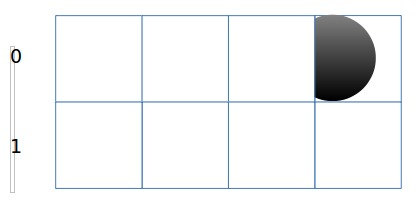
\includegraphics[scale=.5]{image/ppi}
%  \end{center}
%  \caption{Imagen rotada con puntos en pixeles
%  intermedios.}\label{img:ppi}
%\end{figure}
%
%Si el punto cae entre cuatro posiciones de la matriz, el mecanismo
%para calcular el porcentaje es similar. Por ejemplo, si en la
%coordenada (2.7, 1.1) se quiere guardar el valor 2021, este valor
%queda repartido entre las coordenadas (2, 1), (2, 2), (3, 1) y (3, 2).
%El porcentaje asignado se calcula de la siguiente manera: 
%
%\begin{enumerate}[a]
%  \item Ver el porcentaje a asignar por filas y por columnas, es decir,
%    si analizamos la coordenada (2.7, 1.1) desde el punto de vista
%    fila, tendremos un 70\% de 2021 en la fila 3, y un 30\% para la fila
%    2, y si vemos el porcentaje respecto a las columnas, tendremos un
%    10\% de 2021 para la columna 2, y un 90\% para la columna 1.
%  \item Finalmente cruzar la información, y la multiplicación de esos
%    porcentajes, coorresponde a la asignación de 2021 en esa posición.
%\end{enumerate}
%
%Calculando lo antes expuesto se tiene que:
%
%\begin{itemize}
%  \item El 30\% del 90\% de 2021 se guarda en la posición (2, 1), que es igual
%    a 545.67.
%  \item El 30\% del 10\% de 2021 se guarda en la posición (2, 2), que es igual
%    a 60.63.
%  \item El 70\% del 90\% de 2021 se guarda en la posición (3, 1), que es igual
%    a 1273.23.
%  \item El 70\% del 10\% de 2021 se guarda en la posición (3, 2), que es igual
%    a 141.47.
%\end{itemize}
%
%Sumando las cantidades asignadas podemos notar que da 2021. La
%Fig.~\ref{img:punto4pos}, refleja gráficamente esta situación.
%
%\begin{figure}[ht!]
%  \begin{center}
%    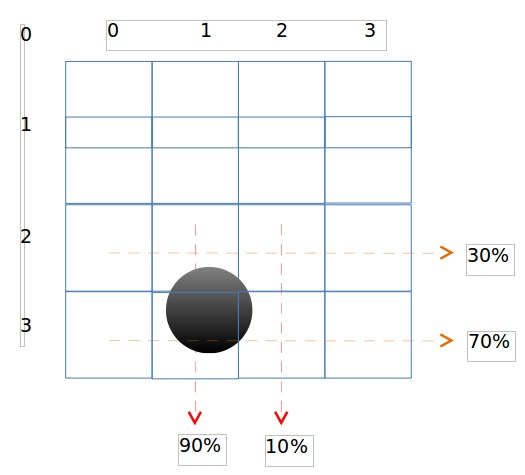
\includegraphics[scale=.5]{image/p4p}
%  \end{center}
%  \caption{Figura rotada con puntos entre 4
%  posiciones.}\label{img:punto4pos}
%\end{figure}
%
%El sentido de repartir la información, es que en un arreglo
%bidimensional no existen posiciones con valores decimales, entonces se
%debe distribuir proporcionalmente la información entre posiciones
%enteras. Puede ocurrir, que en la posición que se asigna el valor,
%tenga previamente información guardada, en este caso tan solo se
%adiciona.
%
%El Alg.~\ref{alg:porcentajes} en pseudo código determina los
%porcentajes asignados según las filas y columnas que contienen al
%punto.
%
%\begin{algorithm}
%\caption{Algoritmo para determinar la medida del arreglo bidimensional
%que contendrá la imagen de la matriz rotada.}\label{alg:porcentajes}
%\label{alg:porcentajes}
%\begin{algorithmic}[1]
%\FOR{$x$ in range(NAXIS1)}
%\FOR{$y$ in range(NAXIS2)}
%\STATE bandera\_decimal\_a = 100
%\STATE bandera\_decimal\_b = 100
%\STATE \#------ Los valores de $a$ y $b$, corresponden a la coordenada (x,y) rotada ------\#
%\IF{$a$ - int($a$) $!= 0$}
%\STATE bandera\_decimal\_a = 101
%\ENDIF
%\IF{$b$ - int($b$) $!= 0$)}
%\STATE bandera\_decimal\_b = 110
%\ENDIF
%\STATE \#------ Esto es un swith() hecho artesanalmente ------\#
%\STATE suma\_banderas = bandera\_decimal\_a + bandera\_decimal\_b
%\STATE \#------ abs() es una function que calcula el valor absolute ------\#
%\STATE \#------ int() calcula el valor entero de un número ------\#
%\WHILE{(1)}
%\STATE porcentaje\_columna\_derecha = porcentaje\_columna\_izquierda = 0
%\STATE porcentaje\_fila\_abajo = porcentaje\_fila\_arriba = 0
%\STATE porcentaje\_fila\_arriba = abs(abs($a$) - int(abs($a$)))
%\STATE porcentaje\_fila\_abajo  = 1 - porcentaje\_fila\_arriba
%\STATE porcentaje\_columna\_derecha = abs(abs($b$) - int(abs($b$)))
%\STATE porcentaje\_columna\_izquierda = 1 - porcentaje\_columna\_derecha
%\ENDWHILE
%\ENDFOR
%\ENDFOR
%\end{algorithmic}
%\end{algorithm}
%
%Hasta el momento, solo se ha extraído información de la coordenada
%rotada que se quiere posicionar, es decir, los porcentajes
%involucrados en la repartición. El código restante (\ref{alg:cruce})
%realiza el cruce de información según la cantidad de valores decimales
%contenidos en la posición, por ejemplo, si el valor 3247 se quiere
%guardar en la coordenada ($a$, $b$), el algoritmo determinará en
%cuantas posiciones repartir el valor según $a$ o $b$ sean decimales.
%
%\begin{algorithm}
%\caption{Algoritmo para realizar el cruce de información según la
%cantidad de valores decimales contenidos en la posición.}\label{alg:cruce}
%\label{alg:cruce}
%\begin{algorithmic}[1]
%\STATE \#------ Solo A es decimal. Ceil (), función que redondea al entero siguiente ------\#
%\IF{suma\_banderas == 201}
%\STATE matriz\_final[int($a$)][$b$] += porcentaje\_fila\_abajo * matriz[$x$][$y$]
%\STATE matriz\_final[ceil($a$)][$b$] += porcentaje\_fila\_arriba * matriz[$x$][$y$]
%\STATE break
%\ENDIF
%\STATE \#------ Solo B es decimal ------\#
%\IF{suma\_banderas == 210}
%\STATE matriz\_final[$a$][int($b$)] += porcentaje\_columna\_izquierda * matriz[$x$][$y$]
%\STATE matriz\_final[$a$][ceil($b$)] += porcentaje\_columna\_derecha * matriz[$x$][$y$]
%\STATE break
%\ENDIF
%\STATE \#------ Ambos son decimales ------\#
%\IF{suma\_banderas == 211}
%\STATE matriz\_final[int($a$)][int($b$)] += porcentaje\_fila\_abajo * porcentaje\_columna\_izquierda * matriz[$x$][$y$]
%\STATE matriz\_final[ceil($a$)][ceil($b$)] += porcentaje\_fila\_arriba * porcentaje\_columna\_derecha * matriz[$x$][$y$]
%\STATE matriz\_final[int($a$)][ceil($b$)] += porcentaje\_fila\_abajo * porcentaje\_columna\_derecha * matriz[$x$][$y$]
%\STATE matriz\_final[ceil($a$)][int($b$)] += porcentaje\_fila\_arriba * porcentaje\_columna\_izquierda * matriz[$x$][$y$]
%\STATE break
%\ENDIF
%\STATE \#------ Ambos son enteros \#------
%\IF{suma\_banderas == 200}
%\STATE matriz\_final[$a$][$b$] = matriz[$x$][$y$]
%\STATE break
%\ENDIF    
%\STATE retorne matriz\_final
%\end{algorithmic}
%\end{algorithm}
%
%La base de este algoritmo es identificar que posiciones, al rotar la
%imagen, quedan en un valor decimal, de esta manera se ve en cuantas
%casillas repartir el valor a posicionar. Para esto se definen dos
%banderas, cada una con un valor 100, entonces cuando el valor en $x$
%es decimal se le asigna el valor 101 a la ‘bandera\_x’, si el valor de
%$y$ es decimal se le asigna a la ‘bandera\_y’ el valor 110, de esta
%manera si la suma de las bandera da 201, significa que tan solo $x$ es
%decimal, si suman 210 significa que tan solo $y$ es decimal, si suman
%211 significa ambos son decimales y si suman 200 significa que ambos
%son números enteros. De esta manera se sabe cuantas casillas se le
%asigna un porcentaje del valor a guardar.
%
%\paragraph{Algoritmo de escalamiento (Alg.~\ref{alg:escalamiento})}
%
%Escalar es agrandar o achicar una imagen en un factor determinado.
%Para escalar una imagen se necesita saber la razón de escala, es
%decir, cuánto más grande o más pequeña es el eje mayor de la imagen
%actual con respecto a la imagen de referencia. Una vez identificado el
%valor, se procede a multiplicar cada coordenada de la matriz por este
%factor (Ec.~\ref{eq:escalamiento}), permitiendo distribuir los puntos
%uniformemente dentro del plano. Si el factor de escala es un número
%entero, quedan puntos intermedios sin información, dado esto, deben
%ser formados a partir de los cuatro puntos mas cercanos. En caso de
%que el propósito sea achicar la imagen, no será necesario aplicar lo
%antes expuesto.
%
%\begin{align}
%  \left[X_2,Y_2\right] & = \left[X_1 * \text{factor}, Y_2 *
%  \text{factor}\right] \label{eq:escalamiento}
%\end{align}
%
%El algoritmo recorre cada posición de la matriz y en la posición
%resultante, que es la posición original por el factor de escala,
%guarda el valor de la posición original. Esto se realiza siempre y
%cuando se necesite expandir la imagen, si el tamaño actual es igual al
%original, no es necesario llevar a cabo esta tarea.
%
%\begin{algorithm}
%\caption{Algoritmo de escalamiento.}\label{alg:escalamiento}
%\label{alg:escalamiento}
%\begin{algorithmic}[1]
%\STATE Función escalar(matriz, NAXIS1, NAXIS2, razón):
%\IF{razón == 1}
%\STATE retornar matriz
%\WHILE{$x$ distinto NAXIS1}
%\WHILE{$y$ distinto NAXIS2}
%\STATE matriz\_final[$x$ * razón][$y$ * razón] = matriz[$x$][$y$]
%\ENDWHILE
%\ENDWHILE
%\ENDIF
%\end{algorithmic}
%\end{algorithm}
%
%Luego de escalar la imagen y solo en caso de que se haya agrandado, se
%debe interpolar, es decir, completar la información faltante a partir
%de los puntos cercanos. Los puntos a considerar no se ven respecto al
%punto vacío, sino que a partir de los cuatro puntos con información se
%rellenan todos los puntos intermedios (Ec.~\ref{eq:interpolar}), esto
%es mas sencillo de diseñar, ya que desde un punto con información a
%otro, la distancia es igual al valor de la razón de escala. El valor
%asignado a la posición sin información corresponde a un porcentaje de
%los cuatro vecinos con información mas cercanos, donde la distancia
%determina su peso. Por ejemplo, si se tuviera cuatro cargas eléctricas
%(a, b, c y d) formando un cuadrado (todas de igual magnitud), y un
%ente conductor se somete a este campo magnético, dependiendo de donde
%este ubicado el ente, se puede determinar la fuerza con que es atraido
%por las cargas. Por ejemplo, en la Fig.~\ref{img:enteCentrado}, hay un
%cilindro centrado en una superficie plana, entre las cargas Q1, Q2, Q3
%y Q4. En este caso, cada carga influye un 25\% de su fuerza sobre el ente.
%
%\begin{align}
%  \text{valor} & = (x, y) * a + (x + \text{razón}, y) * b + (x, y +
%  \text{razón}) * c + (x + \text{razón}, y + \text{razón}) * d
%  \label{eq:interpolar}
%\end{align}
%
%\begin{figure}[hb!]
%  \begin{center}
%    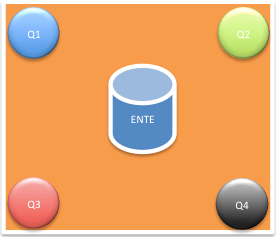
\includegraphics[scale=.5]{image/enteCentrado}
%  \end{center}
%  \caption{Ente conductor sometido a 4 cargas eléctricas de igual
%  magnitud.}\label{img:enteCentrado}
%\end{figure}
%
%Si el ente se desplaza a otra posición, la forma en que cada carga
%influye sobre el ente cambia y se debe considerar la distancia como
%una referencia. La Fig.\ref{img:enteNoCentrado}, muestra un ente que
%está muy apegado a la carga Q4. En este caso, la carga Q4 influye
%mayoritariamente sobre el ente, en menor grado las cargas Q2 y Q3, y
%finalmente, con un porcentaje muy bajo la carga Q1.
%
%\begin{figure}[hb!]
%  \begin{center}
%    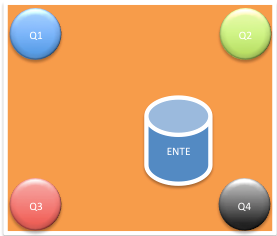
\includegraphics[scale=.5]{image/enteNoCentrado}
%  \end{center}
%  \caption{Ente conductor sometido a 4 cargas eléctricas de igual
%  magnitud.}\label{img:enteNoCentrado}
%\end{figure}
%
%Para determinar el porcentaje asignado a cada carga, se suman todas
%las distancia entre cada carga y el ente, y luego se divide cada
%distancia individual por el total. De esta manera, el valor
%encontrado, se le asigna a la carga del frente. Por ejemplo, si la
%suma de todas las distancia individuales da 10 unidades, y la
%distancia individual de Q1 al ente es 6 unidades, significa que Q4
%influye un 60\% sobre el ente.
%
%Para el ejemplo expuesto, cada carga corresponde a un vecino con
%información, y el ente es una posición de la matriz sin información.
%Como la imagen posee puntos con información igualmente distribuida,
%los porcentajes determinados para las posiciones sin información para
%los cuatro primeros vecinos, es constante para el resto de la imagen.
%En la Fig.\ref{img:m01}, se tiene una matriz con un punto ubicado en
%la posición (0, 1), el cual posee un x1\% de h1, un x2\% de h2, un
%x3\% de h3 y un x4\% de h4. Para todos los puntos ubicados en la
%posición (0, 2$i$), con $i$ pertenecientes a los enteros positivos, le
%corresponderá la misma proporción.
%
%\begin{figure}[hb!]
%  \begin{center}
%    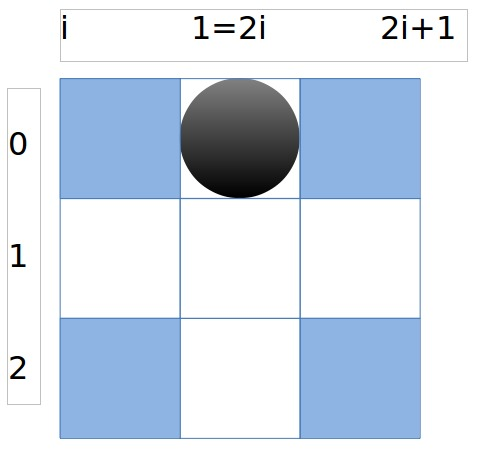
\includegraphics[scale=.5]{image/m01}
%  \end{center}
%  \caption{Matriz ubicada con un punto en la posición (0, 1).}\label{img:m01}
%\end{figure}
%
%El Alg.~\ref{alg:interpolacion} muestra la manera en que se realiza la
%interpolación.
%
%\begin{algorithm}
%\caption{Algoritmo de interpolación.}\label{alg:interpolacion}
%\label{alg:escalamiento}
%\begin{algorithmic}[1]
%\STATE porcentajes = [ ] \#------ Vector dinámico ------\#
%\WHILE{$i$ in range(razon + 1)}
%\WHILE{$j$ in range(razon + 1)}
%\IF{$i$ == 0 AND $j$ == 0 OR $i$ == 0 AND $j$ == razón OR $i$ == razón AND $j$ == 0 OR $i$ == razón AND $j$ == razón}
%\STATE continue
%\ELSE
%\STATE suma\_distancias = info\_imagen.distancia($i$,$j$,0,0) + info\_imagen.distancia($i$,$j$,razon,0) + info\_imagen.distancia($i$,$j$,0,razon) + info\_imagen.distancia($i$,$j$,razon,razon)
%\STATE porcentajes.append(info\_imagen.distancia($i$,$j$,razon,razon)/suma\_distancias)
%\STATE porcentajes.append(info\_imagen.distancia($i$,$j$,razon,0)/suma\_distancias)
%\STATE porcentajes.append(info\_imagen.distancia($i$,$j$,0,razon)/suma\_distancias)
%\STATE porcentajes.append(info\_imagen.distancia($i$,$j$,0,0)/suma\_distancias)
%\ENDIF
%\ENDWHILE
%\ENDWHILE
%\STATE posicion\_vector = 0
%\WHILE{$x <$ (NAXIS1 - 1) * razón}
%\WHILE{$y <$ (NAXIS2 - 1) * razón}
%\STATE pos = [$x$, $y$, $x$ + razon, $y$, $x$, $y$ + razon, $x$ + razon, $y$ + razon]
%\WHILE{$i$ in range($x$, $x$ + razon + 1)}
%\WHILE{$j$ in range($y$, $y$ + razon + 1)}
%\IF{$i$ == pos[0] AND $j$ == pos[1] OR $i$ == pos[2] AND $j$ == pos[3] OR $i$ == pos[4] AND $j$ == pos[5] OR $i$ == pos[6] AND $j$ == pos[7]}
%\STATE continue
%\ENDIF
%\STATE matriz\_final[$i$][$j$] = matriz[$x$][$y$] * porcentajes[posicion\_vector] + matriz[$x$][$y$ + razon - 1] * porcentajes[posicion\_vector+1] + matriz[$x$ + razon - 1][$y$] * porcentajes[posicion\_vector+2] +  matriz[$x$ + razon - 1][$y$ + razon - 1] * porcentajes[posicion\_vector+3]
%\STATE posicion\_vector += 4
%\ENDWHILE
%\ENDWHILE
%\STATE $y$ = $y$ + razón
%\ENDWHILE
%\STATE $y$ = 0
%\STATE $x$ = $x$ + razón
%\ENDWHILE
%\STATE retorne matriz\_final
%\end{algorithmic}
%\end{algorithm}
%
%El Alg.~\ref{alg:interpolacion} posee dos partes vitales, primero, de
%la linea 7 a la 11, determina como queda particionada la posición sin
%información, y segundo, de la linea 15 a la 31, extiende y aplica este
%cáculo al resto de la información.
%
%\paragraph{Algoritmo de alineación}
%
%Alinear geométricamente representa el desplazamiento de un punto o un
%conjunto de puntos según un vector fijo no nulo. El proceso de alinear
%consiste en llevar el centro del objeto de estudio a punto de
%referencia común, con el fin que todos los objetos en cada imagen
%tenga la misma posición antes de ser analizados. Como la imagen que
%está siendo procesada ya posee el mismo tamaño y rotación que la de
%referencia, se puede trasladar tranquilamente el objeto a ese punto,
%sin preocuparse de que la información quede fuera de los márgenes.
%
%Si la imagen de referencia es más pequeña que la actual, al desplazar
%los puntos, solo aquellos que estén dentro de la dimensión de la
%imagen de referencia quedarán guardados. El resto, al no poseer
%información, serán descartados automáticamente. Cuando la imagen de
%referencia es más grande, se traspasará la información completamente
%sin descartar puntos.
%
%Para determinar el vector de traslación, se calcula la distancia en
%$x$ y en $y$, entre el punto de referencia y el punto centro actual,
%de esta manera, los valores son desplazado en esa distancia. La
%Fig.~\ref{img:puntoDesplazado} grafica un ejemplo de un punto que debe
%ser desplazado 1 unidades en $x$, y 2 unidades en $y$.
%
%\begin{figure}[hb!]
%  \begin{center}
%    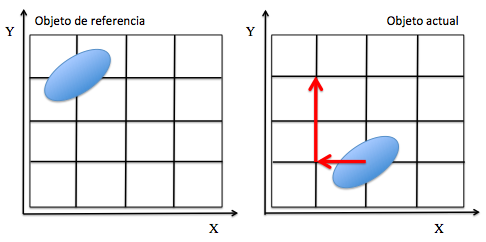
\includegraphics[scale=.5]{image/pd}
%  \end{center}
%  \caption{Traslación de un objeto en el plano $(x,y)$}\label{img:puntoDesplazado}
%\end{figure}
%
%La función alinear no necesita interpolar la información dado que el
%vector de traslación, tiene valores enteros, entonces la posición
%resultante siempre cae en una posición entera.
%
%\begin{algorithm}
%\caption{Algoritmo de interpolación.}\label{alg:interpolacion}
%\label{alg:escalamiento}
%\begin{algorithmic}[1]
%\STATE Función alinear($x1$, $y1$, $x2$, $y2$, dim\_1\_$x$, dim\_1\_$y$, dim\_2\_$x$, dim\_2\_$y$, actual): 
%\STATE diferencia\_$x$ = $x1$ - $x2$
%\STATE diferencia\_$y$ = $y1$ - $y2$
%\WHILE{$i$ distinto dim\_2\_$x$}
%\WHILE{$j$ distinto dim\_2\_$y$}
%\STATE $x$ = $i$ + diferencia\_$x$
%\STATE $y$ = $j$ + diferencia\_$y$
%\IF{$x > 0$ AND $x <$ dim\_1\_$x$ AND $y > 0$ AND $y <$ dim\_1\_$y$)}
%\STATE matriz\_final[$x$][$y$] = actual[$i$][$j$]
%\ENDIF
%\ENDWHILE
%\ENDWHILE
%\STATE retornar matriz\_final
%\end{algorithmic}
%\end{algorithm}
%
%\paragraph{Algoritmo de deproyección}
%
%Es el proceso por el cual se cambia la perspectiva en que se ve un
%objeto. Si pusiéramos las imágenes  en un plano tridimensional ($x$, $y$,
%$z$), siendo $z$ la coordenada que da la profundidad, se apreciaría que
%el ángulo de inclinación respecto al eje varía en cada imagen, lo que
%también se podría llamar perspectiva. Para poder comparar
%correctamente las imágenes es necesario dejar todos los objetos
%paralelos al plano ($x$, $y$).
%
%La Fig.~\ref{img:andromeda} y la Fig.~\ref{img:sombrero} muestra como
%dos galaxias espirales recrean esta misma situación, por un lado una
%está más recostada, destacando más su canto, en cambio en la otra, es
%mas visible su centro y su extensión.
%
%\begin{figure}[hb!]
%  \begin{center}
%    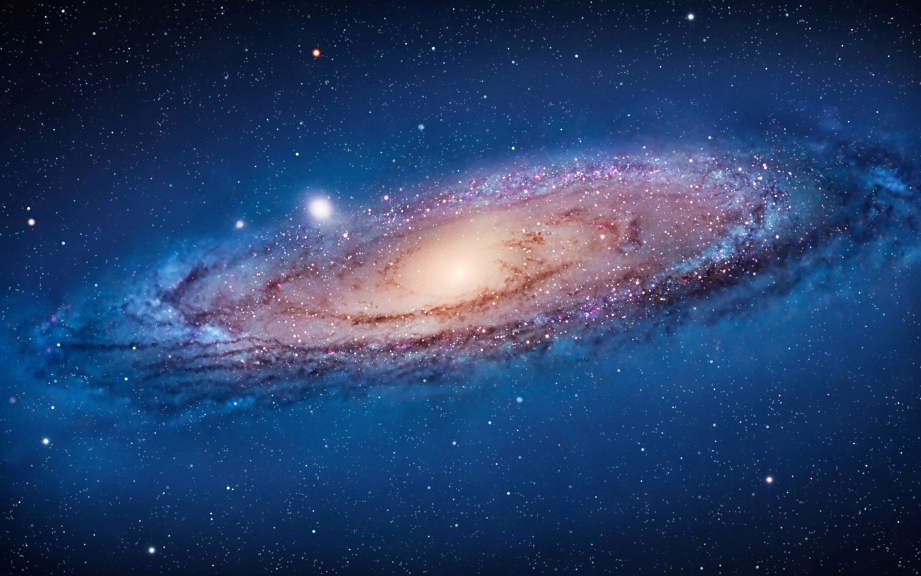
\includegraphics[scale=1]{image/andromeda}
%  \end{center}
%  \caption{Galaxia espiral Andrómeda}\label{img:andromeda}
%\end{figure}
%
%\begin{figure}[hb!]
%  \begin{center}
%    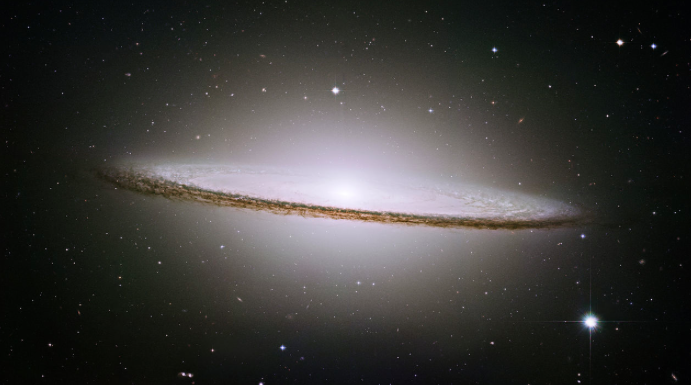
\includegraphics[scale=.5]{image/sombrero}
%  \end{center}
%  \caption{Galaxia espiral ``sombrero''}\label{img:sombrero}
%\end{figure}
%
%Para corregir esta situación, es necesario dejar ambos objetos bajo el
%mismo enfoque, es decir, cambiar el ángulo del objeto en relación a un
%tercer eje. Lamentablemente esto no es factible, dado que no existe
%una tercera coordenada. Para lograr un efecto similar, la elipse se
%puede ‘estirar’ de forma tal, que manteniendo el mismo eje mayor de la
%elipse, se trasforme en un círculo, es decir, encontrar una relación
%entre un punto de la elipse y un punto del círculo. En la
%Fig.~\ref{img:proyPunto} tenemos un círculo con una elipse inscrita,
%compartiendo el mismo diámetro.
%
%\begin{figure}[hb!]
%  \begin{center}
%    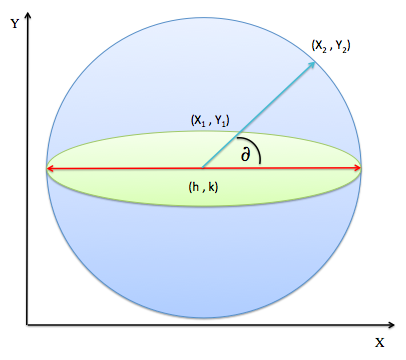
\includegraphics[scale=.5]{image/proyeccion}
%  \end{center}
%  \caption{Proyección de un punto elipse a la circunferencia.}\label{img:proyPunto}
%\end{figure}
%
%Podemos notar que tanto $(X1,Y1)$ e $(X2,Y2)$ comparten el mismo ángulo,
%es decir sabiendo el ángulo compartido y la distancia de cada punto al
%centro geométrico del cuerpo, se podría determinar la coordenada
%equivalente en el circulo. Como el punto $(X1,Y1)$ y el centro $(h,k)$ es
%conocido, aplicando propiedades trigonométricas sencillas se puede
%obtener el ángulo. 
%
%Supongamos que la distancia del punto $(h,k)$ a un punto $(X,Y)$ de la
%elipse mide $a$, y trazando una perpendicular desde ese punto al eje
%horizontal de largo $Y – k$, se estaría formando un triángulo rectángulo
%donde $Y – k$, es el cateto opuesto y $a$, es la hipotenusa, situación
%graficada en la Fig.~\ref{img:triaElipse}.
%
%\begin{figure}[hb!]
%  \begin{center}
%    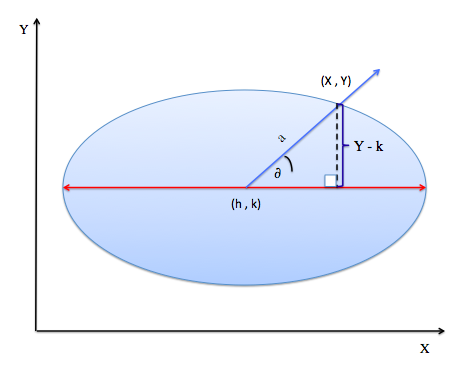
\includegraphics[scale=.5]{image/triaElipse}
%  \end{center}
%  \caption{Catetos e hipotenusa de un triangulo rectángulo inscrito en
%  una elipse.}\label{img:triaElipse}
%\end{figure}
%
%Para determinar el ángulo $\partial$, se calcula el arcoseno de la razón entre
%el cateto opuesto al ángulo con la hipotenusa (Ec.~\ref{eq:arcs}).
%
%\begin{align}
%  \partial & = \sin^{-1}\left(\frac{Y - k}{a}\right) \label{eq:arcs}
%\end{align}
%
%Este ángulo es vital para encontrar el punto equivalente en el
%círculo, ya que teniendo la distancia, que en el caso de un punto
%borde es igual al radio, y escribiendo el punto del círculo en forma
%paramétrica se puede obtener la coordenada. La expresión de a
%continuación (Ec.~\ref{eq:parametrica}), representa la forma
%paramétrica de un punto $(x,y)$.
%
%\begin{align}
%  (x,y) & = (dcos(x), dsen(x)) \label{eq:parametrica}
%\end{align}
%
%Remplazando el ángulo encontrado a partir del punto en la elipse y la
%distancia del centro del cuerpo al punto proyectado, se obtiene la
%coordenada dentro del círculo. Esta distancia varía según el punto,
%pero se determina en relación al punto mayor que está a distancia de
%un radio.  Lamentablemente, este escenario cambia un poco en el ámbito
%computacional, ya que el primer cuadrante del plano cartesiano no es
%equivalente al plano matricial de una imagen, sino más bien es
%similar. Primero, el plano cartesiano tiene el punto (0,0) en el
%origen, en cambio en una imagen el (0,0) se encuentra en la primera
%posición de la esquina superior de la matriz, como lo vemos en la
%Fig.~\ref{img:elipse} y Fig.~\ref{img:matrizElipse}.
%
%\begin{figure}[hb!]
%  \begin{center}
%    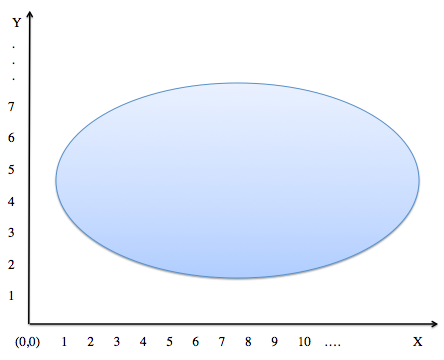
\includegraphics[scale=.5]{image/elipse}
%  \end{center}
%  \caption{Elipse posesionada en el primer cuadrante de un plano
%  cartesiano.}\label{img:elipse}
%\end{figure}
%
%\begin{figure}[hb!]
%  \begin{center}
%    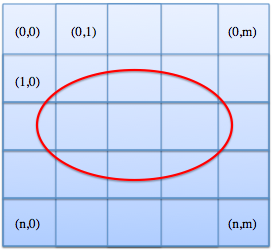
\includegraphics[scale=.5]{image/matrizElipse}
%  \end{center}
%  \caption{Representación matricial de una elipse en un arreglo
%  bidimensional.}\label{img:matrizElipse}
%\end{figure}
%
%Esto cambia completamente la forma de aplicar las funciones
%trigonométricas al plano normal dado que la coordenada $(x,y)$
%representada en una ``matriz computacional'' se lee $(y,x)$, entonces
%la expresión paramétrica del círculo también se escribe al revés
%(Ec.~\ref{eq:circParamatrico}). Otro aspecto a considerar, es la forma
%de leer el ángulo, en el plano cartesiano se hace en sentido
%antihorario, Fig.~\ref{img:planoCartesiano}, pero en este caso se hace
%en sentido horario, \ref{img:planoHorario}, también por el mismo motivo.
%
%\begin{align}
%  (x,y) & = (dsen(x), dcos(x)) \label{eq:circParamatrico}
%\end{align}
%
%\begin{figure}[hb!]
%  \begin{center}
%    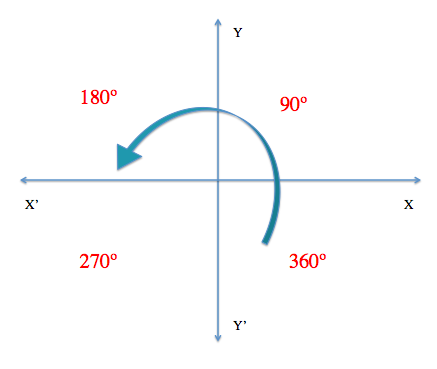
\includegraphics[scale=.5]{image/planoCartesiano}
%  \end{center}
%  \caption{Medición de grados en un plano cartesiano con centro en (0,0).}\label{img:planoCartesiano}
%\end{figure}
%
%\begin{figure}[hb!]
%  \begin{center}
%    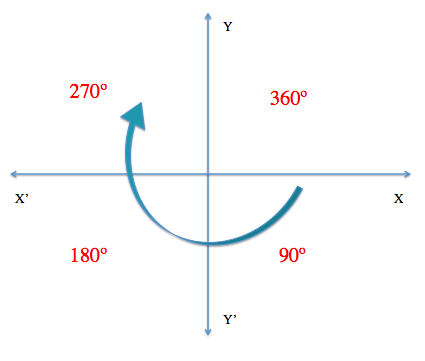
\includegraphics[scale=.5]{image/planoHorario}
%  \end{center}
%  \caption{Medición de grados en un arreglo bidimensional con centro
%  en $(n/2,m/2)$.}\label{img:planoHorario}
%\end{figure}
%
%Teniendo claro esta relación ya es posible proyectar los puntos
%correctamente. El Alg.~\ref{alg:deproyectar} que se presenta, refleja
%la manera en que se elije un punto de la elipse y en base al ángulo
%que posee se proyecta hacia el círculo. Éste recibe como parámetro de
%entrada el centro geométrico del objeto, la dimensión de la imagen
%NAXIS1, NAXIS2, un vector con información de las coordenadas del borde
%del objeto, la matriz de información del objeto y el radio de la
%circunferencia, que sería la mitad del eje mayor de la elipse.
%
%\begin{algorithm}
%\caption{Algoritmo de deproyección.}
%\label{alg:deproyectar}
%\begin{algorithmic}[1]
%\STATE Función deproyectar($x$, $y$, NAXIS1, NAXIS2, borde, matriz, radio):
%\WHILE{$i$ != NAXIS1}
%\WHILE{$j$ != NAXIS2}
%\STATE $a = b = c = d = 0$
%\WHILE{$r$ != largo(borde - 1)}
%\IF{($r$ es impar)}
%\STATE continúe
%\ENDIF
%\IF{$i <$ borde[$r$]}
%\STATE $a = 1$
%\ENDIF
%\IF{$i >$ borde[$r$]}
%\STATE $b = 10$
%\ENDIF
%\IF{$j >$ borde[$r + 1$]}
%\STATE $c = 100$
%\ENDIF
%\IF{$j <$ borde[$r + 1$]}
%\STATE $d = 1000$
%\ENDIF
%\IF{$i$ == borde[$r$] AND $j$ == borde[$r + 1$]}
%\STATE $a,b,c,d$ = 1,10,100,1000
%\STATE break
%\ENDIF
%\ENDWHILE
%\IF{($a + b + c + d$ != 1111 OR $x == i$ AND $y == j$)}
%\STATE continúe
%\ENDIF
%\STATE ángulo = arcoseno(($j - y$)/distancia($x,y,i,j$))
%\WHILE{TRUE}
%\IF{$i > x$ AND $j > y$}
%\STATE ángulo = ángulo
%\STATE break
%\ENDIF
%\IF{$i < x$ AND $j > y$}
%\STATE ángulo = 360 – ángulo
%\STATE break
%\ENDIF
%\IF{$i < x$ AND $j < y$}
%\STATE ángulo = 180 + ángulo
%\STATE break
%\ENDIF
%\IF{$i > x$ AND $j < y$}
%\algstore{myalg}
%\end{algorithmic}
%\end{algorithm}
%
%
%\begin{algorithm}
%\begin{algorithmic}[1]
%\algrestore{myalg}
%\STATE ángulo = 180 – ángulo
%\STATE break
%\ENDIF
%\IF{$i == x$ AND $j > y$}
%\STATE ángulo = 0
%\STATE break
%\ENDIF
%\IF{$i == x$ AND $j < y$}
%\STATE ángulo = 180
%\STATE break
%\ENDIF
%\IF{$i > x$ AND $j == y$}
%\STATE ángulo = 90
%\STATE break
%\ENDIF
%\IF{$i < x$ AND $j == y$}
%\STATE ángulo = 270
%\STATE break
%\ENDIF
%\ENDWHILE
%\ENDWHILE
%\STATE fil = $x$ + (seno(ángulo * 3.14/180)) * distancia
%\STATE col = $y$ + (coseno(ángulo * 3.14/180)) * distancia
%\ENDWHILE
%\STATE matriz\_final[fil,col] = matriz[$i$][$j$]
%\STATE retornar matriz\_final
%\end{algorithmic}
%\end{algorithm}
%
%La clave de este algoritmo es determinar que puntos pertenecen al
%objeto antes de desplazar. Para esto se puede establecer lo siguiente:
%todo punto perteneciente al objeto va a estar entre cuatro puntos a
%menos que sea el borde de este. Por esta razón, el algoritmo parte
%recorriendo toda la matriz imagen hasta detectar un punto objeto. Una
%vez localizado se calcula el ángulo relacionado, el cual siempre va a
%estar entre 0 y 90 grados, ya que se calcula en base a la distancia
%entre los puntos y el cateto opuesto, por lo que, determinando en qué
%parte del plano está en relación al punto $(h,k)$ se le suma lo
%faltante. La Fig.~\ref{img:proyeccionPunto} recrea esta situación.
%Como el punto $(x1,y1)$ a proyectar se encuentra en la esquina
%superior derecha del centro y dado que los ángulos se cuentan en
%sentido antihorario, el ángulo no vale $\partial^\circ$, sino más bien
%360 - $\partial$. Si hubiésemos tomado un punto de la esquina superior
%izquierda, su ángulo sería 180 + $\partial$, si el punto está en la
%parte inferior izquierda 180 - $\partial$, y finalmente si ubiese
%estado en el lado inferior derecha, el ángulo se mantiene. Ya
%determinado el ángulo, el algoritmo ocupando la ecuación paramétrica
%de un punto en el círculo, y calculando brevemente la distancia que
%debería estar el punto en relación al punto más distante, se obtiene
%la coordenada del punto proyectado. Este proceso se repite tantas
%veces como puntos pertenezcan al objeto de estudio. Una vez finalizado
%todo el proceso, se retorna una matriz que posee la proyección de la
%elipse a un círculo.
%
%\begin{figure}[hb!]
%  \begin{center}
%    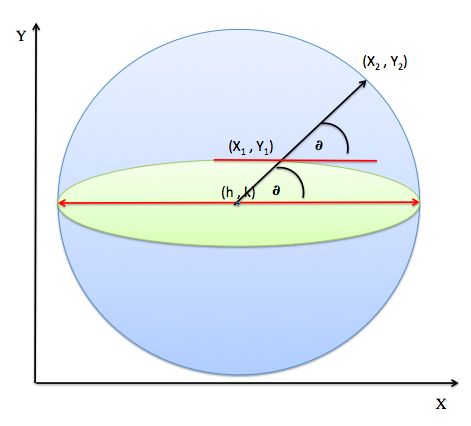
\includegraphics[scale=.5]{image/proyeccionPunto}
%  \end{center}
%  \caption{Proyección de un punto elíptico a un punto del círculo.} \label{img:proyeccionPunto}
%\end{figure}
%
%\subsection{Funciones especiales}
%
%Si bien el registro de imágenes contempla cuatro niveles de ajustes,
%detrás de estos módulos actúan constantemente funciones que entregan
%información valiosa antes de realizar cualquier ajuste a un objeto en
%el plano. Estas funciones son ‘invisibles’ para el usuario, es decir,
%no entregan resultados tangible u observables, sino más bien es el
%sistema de cómputo que aporta información sobre los cuerpos
%geométricos, como tamaño, grado de inclinación y posición, para que
%los módulos que realizan el registro sepan a priori en qué medida
%ajustar el objeto.
%
%\paragraph{Distancia entre puntos}
%
%Para un objeto elíptico posicionado dentro de una imagen es necesario
%medirlo antes de escalarlo, de esta manera se puede determinar que tan
%grande o más pequeño es el objeto de la imagen actual, con la imagen
%de referencia. La medición de un objeto se basa en determinar la
%distancia entre los puntos más distantes pertenecientes al borde de la
%elipse, conocida también como distancia euclidiana, la cual se calcula
%mediante la Ec.~\ref{eq:distanciaEuclidiana}.
%
%\begin{align}
%  d & = \sqrt{\left(x_2 - x_1\right)^2 + \left(y_2 - y_1\right)^2}
%  \label{eq:distanciaEuclidiana}
%\end{align}
%
%La Ec.~\ref{eq:distanciaEuclidiana} indica que la raíz cuadrada de la
%suma de la diferencia de las coordenadas al cuadrado es igual a la
%distancia $d$. Algorítmicamente se ve de como en el
%Alg.~\ref{alg:distanciaEuclidiana}.
%
%\begin{algorithm}
%\caption{Algoritmo de distancia Euclidiana.}
%\label{alg:distanciaEuclidiana}
%\begin{algorithmic}[1]
%\STATE Función distancia (x1, y1, x2, y2):
%\STATE retornar raiz\_cuadrada$((x2 - x1)^2 + (y2 - y1)^2))$
%\end{algorithmic}
%\end{algorithm}
%
%La función recibe como parámetros de entrada el par de coordenadas de
%las cuales se desea saber su distancia, para luego al igual que la
%fórmula anterior retornar la distancia.
%
%\paragraph{Distancia eje mayor}
%
%Esta función no es más que una aplicación de la función distancia, lo
%distinto es que busca la mayor distancia entre todos los puntos que
%componen el borde del objeto elíptico. De esta manera cuando encuentra
%los puntos más distantes, sabe de inmediato que corresponde al eje
%mayor de la elipse. 
%
%La función del Alg.~\ref{alg:distEjeMayor}, recibe como parámetro de
%entrada un arreglo que contiene todas las posiciones del borde de la
%elipse, de las cuales se localizará las más distantes.
%
%\begin{algorithm}
%\caption{Algoritmo de distancia al eje mayor}
%\label{alg:distEjeMayor}
%\begin{algorithmic}[1]
%\STATE Función eje\_mayor(borde):
%\STATE info\_elipse = [0,0,0,0,0]
%\WHILE{$i$ distinto largo(borde) - 2}
%\IF{($i$ es impar)}
%\STATE continúe
%\ENDIF
%\STATE $i = i + 2$
%\WHILE{$j$ distinto largo(borde) - 1}
%\IF{($j$ es impar)}
%\STATE continúe
%\ENDIF
%\STATE dis = distancia(borde[$i$], borde[$i + 1$], borde[$j$], borde[$j + 1$])
%\IF{dis $>$ info\_elipse[0]}
%\STATE info\_elipse[0] = dis          
%\STATE info\_elipse[1] = borde[$i$]     
%\STATE info\_elipse[2] = borde[$i+1$]   
%\STATE info\_elipse[3] = borde[$j$]
%\STATE info\_elipse[4] = borde[$j+1$]
%\ENDIF
%\ENDWHILE
%\ENDWHILE
%\STATE retornar info\_elipse
%\end{algorithmic}
%\end{algorithm}
%
%En la línea número dos, se crea un vector que guardará en su posición
%0 la distancia del eje, y en las posiciones restantes sus coordenadas,
%por ejemplo, si el eje mayor mide 30 unidades, y sus coordenadas son
%$(X1, Y1)$ y $(X2, Y2)$, el vector se escribe como en la
%Ec.~\ref{eq:infoVector}.
%
%\begin{align}
%  \text{info}_{\text{vector}} & = [30, X_1, Y_1, X_2, Y_2]
%  \label{eq:infoVector}
%\end{align}
%
%Este vector es iniciado con ceros, ya que cada posición actúa como una
%variable auxiliar mientras se busca el eje mayor.
%
%Los ciclos \textbf{while} de la línea 3 y 8 permitirán encontrar la mayor
%distancia, para esto el ciclo de la línea 3 va seleccionando una
%coordenada del vector y el ciclo de la línea 8 compara la coordenada
%elegida en el ciclo 3 con todas las coordenadas restantes. Si esta
%resulta ser mayor que la encontrada anteriormente, se reemplaza en la
%posición cero del vector ‘info\_vector’ la distancia encontrada y se
%actualizan las coordenadas de las cuales se extrajo la distancia.
%
%\paragraph{Ángulo a rotar (Alg.~\ref{alg:rotar})}
%
%Para rotar un objeto en el plano es necesario saber cuánto es lo que
%se necesita rotar. La siguiente función determina a partir de la
%información generada anteriormente cuánto es lo que necesita rotarse
%el objeto para que su eje mayor quede paralelo al eje horizontal en un
%plano. 
%
%\begin{algorithm}
%\caption{Algoritmo de ángulo a rotar}
%\label{alg:rotar}
%\begin{algorithmic}[1]
%\STATE Función angulo\_a\_rotar (x1, y1, x2, y2):
%\IF{$(y2 - y1) == 0$}
%\STATE retorne 90
%\ELSE
%\STATE retorne 180 – arcotangente $((y2 - y1)/(x2 - x1))$
%\ENDIF
%\end{algorithmic}
%\end{algorithm}
%
%La función recibe como entrada las coordenadas extremas del eje mayor
%del objeto. En la línea dos pregunta si el eje mayor es paralelo al
%eje $y$, de esta manera se debe rotar, de lo contrario calcula el
%arcotangente del ángulo. En la línea cinco, se le resta esta cantidad
%a 180, esto es debido a que la función que realiza la rotación gira en
%sentido antihorario el cuerpo, por tal motivo, cuando se determina el
%ángulo de la recta se calcula su complemento.
%
%Matemáticamente consiste en determinar la tangente del ángulo
%$\partial$ que forma la recta con la dirección positiva del eje de las
%abscisas, por lo tanto, para determinar el ángulo se realiza el
%proceso inverso (Ec.~\ref{eq:m} y Ec.~\ref{eq:arctm}).
%
%\begin{align}
%  m & = \frac{y_2 - y_1}{x_2 - x_1} \label{eq:m}\\
%  \partial & = \arctan{m} \label{eq:arctm}
%\end{align}
%
%\paragraph{Centro geométrico (Alg.~\ref{alg:centroGeo})}
%
%Al momento de alinear un objeto es necesario determinar su punto
%central para poder trasladar esa coordenada al punto que se tiene como
%referencia. Para poder determinar la coordenada del centro geométrico
%del objeto, se calcula a partir del tamaño de la mitad del eje mayor
%de la elipse, la proyección del ángulo en el eje horizontal y vertical.
%
%\begin{algorithm}
%\caption{Algoritmo para calcular centro geométrico}
%\label{alg:centroGeo}
%\begin{algorithmic}[1]
%\STATE Función centro\_geométrico(dis,x1,y1,x2,y2,angulo):
%\IF{(ángulo $<$ 90)}
%\STATE punto\_central = [$x1$ + 0.5 * coseno(ángulo) * dis, $y1$ + 0.5 * seno(ángulo)*dis]
%\ENDIF
%\IF{(ángulo $> 90$)}
%\STATE punto\_central = [$x2$ - 0.5 * cos(angulo) * dis, $y2$ – 0.5 * seno(ángulo) * dis]
%\ENDIF
%\IF{(ángulo == 90)}
%\STATE punto\_central = [$(x1-x2)/2$ , $y1$]
%\ENDIF
%\STATE retornar punto\_central
%\end{algorithmic}
%\end{algorithm}
%
%La función recibe como parámetro de entrada la medida del eje ‘dis’,
%las coordenadas extremas y el ángulo que corresponde a la pendiente.
%
%La clave de este algoritmo es saber si la pendiente del eje es
%positiva o negativa, ya que la proyección de la recta en los ejes, se
%hace a partir de la coordenada más baja del objeto al punto central,
%por este motivo, se pregunta si el ángulo de la recta es mayor o menor
%que $90^\circ$. Al obtener el punto central del eje, debe sumarse la
%coordenada menor del eje del objeto, esto se hace de esta manera ya
%que el punto centro encontrado es el centro del objeto y no el centro
%del objeto en relación al plano. Por tal motivo en la linea tres y
%cinco del plano se suma $(x1,y1)$ y $(x2,y2)$. Finalmente, se retorna la
%coordenada. 
%
%Estos cuatro últimos algoritmos entregan toda la información necesaria
%para que cada etapa del registro realice correctamente un ajuste de la
%información. Partiendo desde la toma de medidas del objeto de
%referencia, hasta la actualización del mismo en cada etapa.
%

